\input preamble.tex
\begin{centering}
\Huge{\textbf{Høstprøve 01}}\\
\end{centering}
\vskip 2cm 
Kompetansemål som prøven omhandler:
\begin{itemize}
	%\item utføre arbeid på automatiserte anlegg fagmessig, nøyaktig og i overensstemmelse med krav til helse, miljø og sikkerhet og rutiner for kvalitetssikring og internkontroll
	%\item utføre risikovurdering og vurdere tiltak for ivaretakelse av person– og maskinsikkerhet
	%\item vurdere hvilke regelverk og normer som gjelder for arbeidet som skal utføres og anvende dette
	\item planlegge, utføre, vurdere kvalitet, sluttkontrollere og dokumentere arbeidet
	\item planlegge, programmere, montere og idriftsette programmerbare styresystemer
	\item endre og tilpasse skjermbilder for grensesnitt mellom menneske og maskin
	\item anvende ulike elektroniske kommunikasjonssystemer i automatiserte anlegg
	%\item vurdere datasikkerhet i automatiserte anlegg
	\item tegne, lese og forklare instrumenterte prosessflytskjemaer og bruke annen relevant dokumentasjon for automatiserte anlegg
	\item montere, konfigurere, kalibrere og idriftsettelse digitale og analoge målesystemer
	%\item idriftsette og optimalisere regulatorer basert på prosessbehov
	%\item montere og idriftsette ulike typer pådragsorganer med tilhørende forstillingselementer og hjelpeutstyr
	%\item programmere, idriftsette samt gjøre rede for roboters funksjon og anvendelse i produksjonsanlegg
	%\item måle fysiske størrelser i automatiserte anlegg
	%\item feilsøke og rette feil i automatiserte anlegg
	%\item bruke gjeldende regelverk og normer for elektriske installasjoner på maskiner
	%\item bruke gjeldende regelverk og normer for installasjon av elektroniske kommunikasjonssystemer
	%\item beskrive ulike vedlikeholdssystemer og -rutiner knyttet til automatiserte anlegg, og anvende et av disse
	%\item redegjøre for bedriftens organisasjonsoppbygging og bedriftens verdiskapning i et samfunnsperspektiv
	%\item dokumentere egen opplæring i automatiseringssystemer
\end{itemize}

Læringsmål som prøven omhandler:
\begin{itemize}[noitemsep]
\item 		Kunne løse kombinatoriske styringer med PLS programmering. 
\item 		Kunne sette opp modbus master og slave i codesys  
\item 		Kunne bruke modbus til å hente ønskede signaler 
\item 		Kunne gjøre tilkoblinger til PLS med digitale og analoge signaler 
\item 		Kunne tilpasse signaler inn og ut av PLS. 
\item 		Kunne lage en HMI tilpasset PLS programmet.  
\end{itemize}



\vskip 2.5pt 
Hjelpemidler:\begin{itemize}[noitemsep]
	\item Oppgave 1-4: Kalkulator og formelark
	\item Oppgave 5-9 Alle ikke kommuniserende
\end{itemize}

\vskip 5pt 
\vskip 10pt 
Alle ark som leveres inn skal ha elevens navn.
\vskip 2.5pt 
Oppgave 1-4 skal leveres på papir, etter levering kan eleven ta frem PC og svare på oppgave 9. 
\vskip 2.5pt 
Oppgave 5-9 skal utføres i samme codesys project. (slik at det bare leveres inn en fil.)
Når oppgave 5-9 skal leveres kan elevene slå på trådløst nettverkt og sende oppgaven på mail til:
\vskip 2.5pt 
fred-olav.mosdal@skole.rogfk.no
\vskip 2.5pt 
I emnefeltet skal det stå: Høstprøve
\vskip 2.5pt
Oppgaven SKAL sendes fra skolemailen. 
\vskip 2cm   
Konaktinformasjon:
\begin{itemize}[noitemsep]
	\item Kontaktlærer: Fred-Olav Mosdal
	\item TLF: 90507684
\end{itemize}


\vfil \eject
\newpage
\
\newpage
%Slutt forside
Oppgave 1 (6p)%Navngi
\vskip 2.5pt 

Tegn inn de nødvendige koblingene for å koble to nærhetsbrytere og to solid-state releer til en Allen-Bradley MicroLogix 1000 PLC (model 1761-L10BWA, med 6 DI-er som kan være sourcing eller sinking og 4 DO med potensialfrie relekontakter. Koble nærhetsbryteren som er sourcing (PNP) til inngang \texttt{I:I/0}, bryteren som er sinking til \texttt{I:I/4}, og de to solid state-releene til \texttt{O:O/1} og \texttt{O:O/2}:


\vskip 5cm
$$\includegraphics[width=15.5cm]{i04524x01.eps}$$


\vskip 30pt

\vfil\eject
Oppgave 2 (6p) %Definisjoneri
\\
Her vises to transmittere og en I/P konverter som skal kobles til en PLS ved hjelp av en analog inngangmodul og en analog utgangmodul. Begge transmitterne og I/P konverteren bruker 2-leder koblet instrumentsløyfe (4-20mA) brukes til å styre en pneumatisk reguleringsventil. \\

Vis hvordan dette utstyret kan kobles til IO-modulene. 
\vskip 5cm
$$\includegraphics[width=15.5cm]{aAuntom01x01.eps}$$


\vfil\eject

Oppgave 3 (6p)%Enkel utregninger.

\vskip 2.5pt 

Hvilken oppgave har en optokobler på en PLS inngang for digitale signaler. 

\vskip 10pt

\begin{tikzpicture}
	\draw[step=0.5cm,gray!20,thin]  grid (17,16) ;
\end{tikzpicture}
\vskip 10pt 


Oppgave 4 (6p) %Tegneoppgaver(blokkskjema skisse osv. 
Bildet viser en Koyo "CLICK" PLS med tilkoblinger.
$$\includegraphics[width=10cm]{i04666x01.eps}$$

Fastslå status på bryterne (aktivert eller ikke) og om lampen lyser, ut fra online bilde av PLS programmet. 

$$\includegraphics[width=15.5cm]{i04666x02.eps}$$

\vskip 10pt

\begin{tikzpicture}
	\draw[step=0.5cm,gray!20,thin]  grid (17,6) ;
\end{tikzpicture}
\vskip 10pt 

\vskip 10pt 
% Her kommer oppgaver som skal kreve forklaringer eller forståelse
\vfil\eject
Oppgave 5 (6p) %Kombinatorisk programmering

\vskip 2.5pt 
\vskip 2.5pt
 Du skal lage en PLS styring til anlegget nedenfor. Bilder av programmet sammen med eventuelle forklaringer legges inn i et dokument. 
 \vskip 10pt 
$$\includegraphics[width=16cm]{aStyring01x01.eps}$$
\vskip 10pt 
		\begin{enumerate}[label=(\alph*)]
	\item Lag et program for Start og Stopp av transportbåndet. Transportbåndet skal også stopppe ved manglende klar signal fra sikkerhetsrelaterte deler av styresystemet. 
	
	\item Legg til forsinket start på 3s av transportbåndet 
	
		\end{enumerate}

		


\vskip 10pt 
Oppgave 6 (6p) % Tegn og forklar virkemåte
\vskip 2.5pt 
Fortsettelse fra oppgave 5

\begin{itemize}[noitemsep]
	\item Når esken er full (10 deler), skal transportbåndet stoppe og det skal gis signal om at eske er full
	
	\item Om det ikke er registrert ny del på 15s skal transportbåndet stoppe og et varsellys aktiveres. 
\end{itemize}


\vskip 10pt 
Oppgave 7 (6p) % Tegn og forkalr virkemåte. 
\vskip 2.5pt 

Vis, med bilder og forklaringer,  hvordan du kan sette opp PLS programmet til å sende følgende data til HMI med modbus master:

\begin{itemize}[noitemsep]
	\item Antall deler
	\item om båndet går
\end{itemize}
\vskip 10pt 
Oppgave 8 (6p) % Regneoppgave
\vskip 2.5pt 
\vskip 1cm

Fra HMI skal en også kunne forandre følgende:

\begin{itemize}[noitemsep]
	\item Hvor mange deler som tilsvarer full eske
	\item Hvor lang tid det skal ta før båndet uten nye deler. 
\end{itemize}
\vskip 5pt 
Vis, med bilder og forklaringer,  hvordan du kan sette opp PLS programmet til å motta disse signalene.
\vskip 0.5cm


\vfil\eject
Oppgave 9 (12p) \\ %skal beskrive hvordan en jobb skal utføres. (Planlegg, besriv hvordan du ville gjenomført og dokumenter jobben)
Som lærling får du følgende oppgave: \\\\
Tilkobling av en temperaturtransmitter (4-20mA utgang) til en Wago PLS. Det er ikke flere analoge innganger på PLS-en slik at du må også montere en ny AI-modul (750-455). Temperaturtransmitteren er kalibrert med LRV=0°C og URV=50°C. Programmering og tilpassing av HMI slik at temperatur vises med tall på skjermen. 
\\\\
Vis hvordan du ville planlagt, gjennomført og dokumentert jobben.


\vskip 5pt 
\includepdf[pages=-,angle=90]{../eq/afgvformler.pdf}
\end {document}
